\documentclass[dvipsnames]{beamer}
\input{mybeamerdefs}

\begin{document}

\begin{frame}{\today}
\begin{itemize}
\item I simulated diffusion MR giving the ems the diffusion properties of free water to test my DWI-associated routines.
\end{itemize}
\end{frame}

\section{Diffusion MR test}

\begin{frame}{Summary}
\begin{itemize}
\item I defined a pulse sequence with a single 90 degree tipping pulse and a diffusion-weighting gradient in the $x$ direction. The magnitude of the diffusion-weighting gradient determines the ``b value."
\item I ran a simulation with 1000 ems, $D = 3 \times 10^{-9}~\mathrm{m^2/s}$ (diffusion coefficient of free water) in the $x$ direction. No diffusion in the $y$ or $z$ directions.
\item I repeated this simulation for b values in \texttt{linspace}(0,1500,5) and recorded the MR signal magnitude $S(b)$.
\item In theory, the relation between $S(b)$ and $b$ is
\begin{equation*}
S(b) = S(0)\exp(-b \cdot ADC)\,,
\end{equation*}
where $ADC$ is the ``apparent diffusion coefficient." In this case, $ADC$ should be equal to $D$.
\end{itemize}
\end{frame}

\begin{frame}
\begin{center}
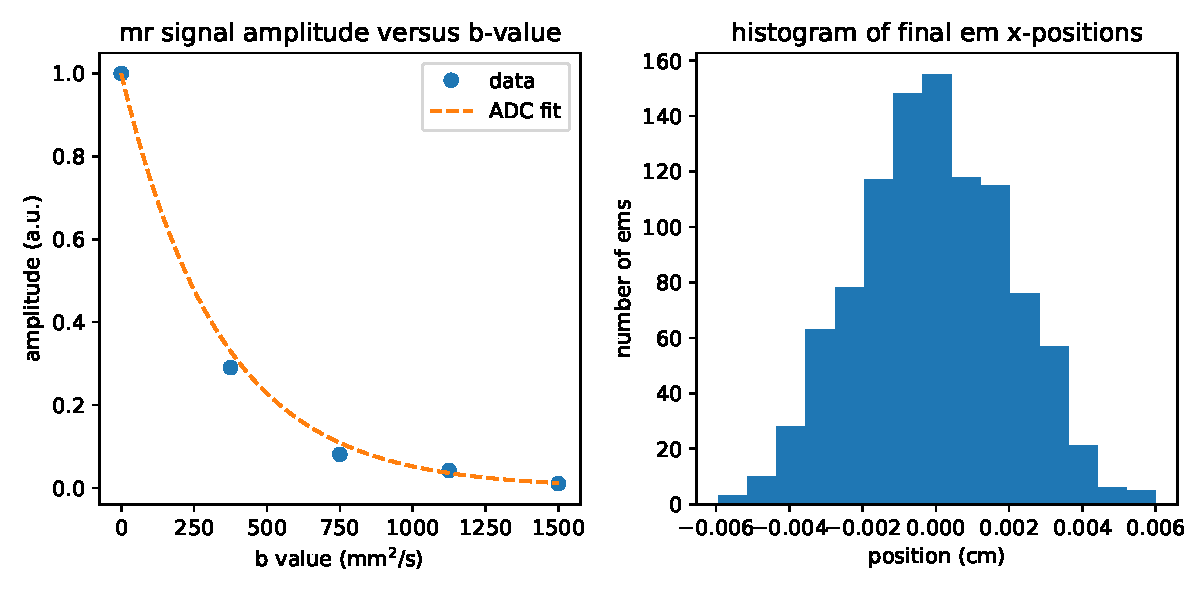
\includegraphics[width=\textwidth]{mr-b_num-ems-1000}
\begin{equation*}
\begin{aligned}
D &= 3 \times 10^{-9}~\mathrm{m^2/s}\\
ADC &= 2.956 \times 10^{-9}~\mathrm{m^2/s}
\end{aligned}
\end{equation*}
\end{center}
\end{frame}

\begin{frame}{Comments}
\begin{itemize}
\item The fitted $ADC$ agrees with $D$, the actual diffusion coefficient.
\item The final em positions look Gaussian. According to the diffusion relation $\sigma = \sqrt{2DT}$, where $T$ is the total diffusion time, the standard deviation of this Gaussian should be $0.0009$ cm, which appears to be an underestimate of the standard deviation of the em distribution, not sure why.
\item The results look reasonable overall.
\end{itemize}
\end{frame}

\end{document}